\begin{figure}[!h]
\centering
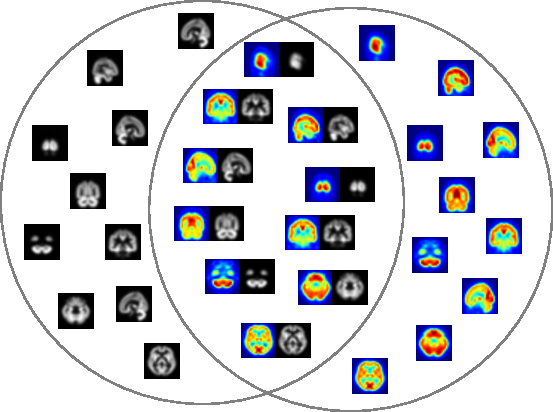
\includegraphics[width=0.8\columnwidth]{./tex/fig/nimg_scheme.pdf}
\caption{
	Pictorial example of training imaging dataset with two views, named \textit{left} and \textit{right} views.
	In this case we have 30 independent observations:
	$10$ with left-views only; $10$ with right-views only; $10$ with complete views.
	The fraction f of observations with complete views is:
	$f = 1/3$.
}
\label{fig:nimg_scheme}
\end{figure}
%
\begin{figure}[!h]
\centering
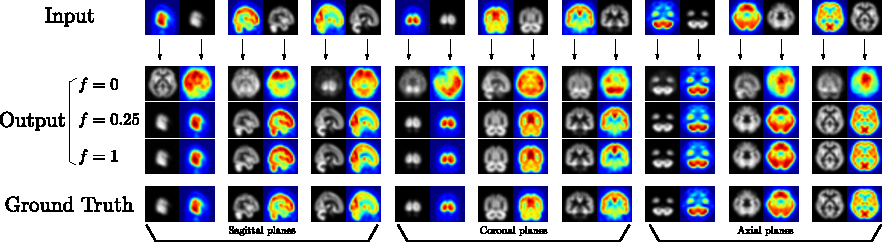
\includegraphics[width=\columnwidth]{./tex/fig/nimg_test.pdf}
\caption{
	Reconstruction of test-set digits when models are trained with an increasing fraction ($f$) of observations with complete-views.
	The left side of each digit is inferred from the input right side and \textit{vice versa}.
}
\label{fig:nimg_test}
\end{figure}
